% !TEX TS-program = pdflatex
% !TEX encoding = UTF-8 Unicode

% This is a simple template for a LaTeX document using the "article" class.
% See "book", "report", "letter" for other types of document.

\documentclass[11pt]{article} % use larger type; default would be 10pt

\usepackage[utf8]{inputenc} % set input encoding (not needed with XeLaTeX)

%%% Examples of Article customizations
% These packages are optional, depending whether you want the features they provide.
% See the LaTeX Companion or other references for full information.

%%% PAGE DIMENSIONS
\usepackage{geometry} % to change the page dimensions
\geometry{letterpaper} % or letterpaper (US) or a5paper or....
\geometry{margin=1in} % for example, change the margins to 2 inches all round
% \geometry{landscape} % set up the page for landscape
%   read geometry.pdf for detailed page layout information

\usepackage{graphicx} % support the \includegraphics command and options
\usepackage{colortbl}
% \usepackage[parfill]{parskip} % Activate to begin paragraphs with an empty line rather than an indent
\usepackage{amssymb}
\usepackage{amsmath}
\usepackage{amsfonts}
\usepackage{bbm}
\usepackage{amsthm}

%%% PACKAGES
\usepackage{booktabs} % for much better looking tables
\usepackage{array} % for better arrays (eg matrices) in maths
\usepackage{paralist} % very flexible & customisable lists (eg. enumerate/itemize, etc.)
\usepackage{verbatim} % adds environment for commenting out blocks of text & for better verbatim
\usepackage{subfig} % make it possible to include more than one captioned figure/table in a single float
% These packages are all incorporated in the memoir class to one degree or another...

%%% HEADERS & FOOTERS
\usepackage{fancyhdr} % This should be set AFTER setting up the page geometry
\pagestyle{fancy} % options: empty , plain , fancy
\renewcommand{\headrulewidth}{0pt} % customise the layout...
\lhead{}\chead{}\rhead{}
\lfoot{}\cfoot{\thepage}\rfoot{}

%%% SECTION TITLE APPEARANCE
\usepackage{sectsty}
\allsectionsfont{\sffamily\mdseries\upshape} % (See the fntguide.pdf for font help)
% (This matches ConTeXt defaults)

%%% ToC (table of contents) APPEARANCE
\usepackage[nottoc,notlof,notlot]{tocbibind} % Put the bibliography in the ToC
\usepackage[titles,subfigure]{tocloft} % Alter the style of the Table of Contents
\usepackage{bbm}
\usepackage{endnotes}
\renewcommand{\qed}{\hfill\blacksquare}
\renewcommand{\cftsecfont}{\rmfamily\mdseries\upshape}
\renewcommand{\cftsecpagefont}{\rmfamily\mdseries\upshape} % No bold!
\DeclareMathOperator*{\argmax}{arg\,max}
\DeclareMathOperator*{\argmin}{arg\,min}
\usepackage{graphicx}
\graphicspath{ {./pings/} }

\newcount\colveccount
\newcommand*\colvec[1]{
	\global\colveccount#1
	\begin{pmatrix}
		\colvecnext
	}
	\def\colvecnext#1{
		#1
		\global\advance\colveccount-1
		\ifnum\colveccount>0
		\\
		\expandafter\colvecnext
		\else
	\end{pmatrix}
	\fi
}

\newcommand{\norm}[1]{\left\lVert#1\right\rVert}

\title{Problem Set \#3\\ ~\\ \large{Econ 899, Fall 2021} }
\author{Heejin Yoon}


\begin{document}
\maketitle
~\\

\section*{Exercise 1}

\begin{itemize}
	\item The value function over the possible asset choices of the age of 50 is drawn below. We can easily see the value function is increasing and concave. 
	
	\begin{center}
		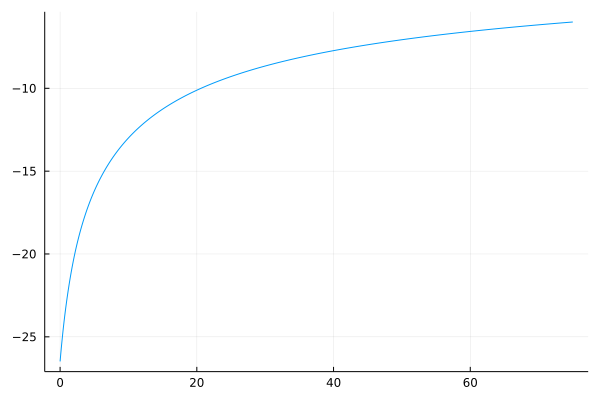
\includegraphics[width=.8\linewidth]{./julia/val_func_50.png}
	\end{center}
	\pagebreak
	\item The savings function of the age of 20 is illustrated as follows. The laws of motions for savings differ by $z$. For $z_{High}$, saving is decreasing in $a$ until the retirement, but increasing after the retirement. For $z_{Low}$, saving is always increasing in $a$, regardless of whether the agent is working or not.
	
	\begin{center}
		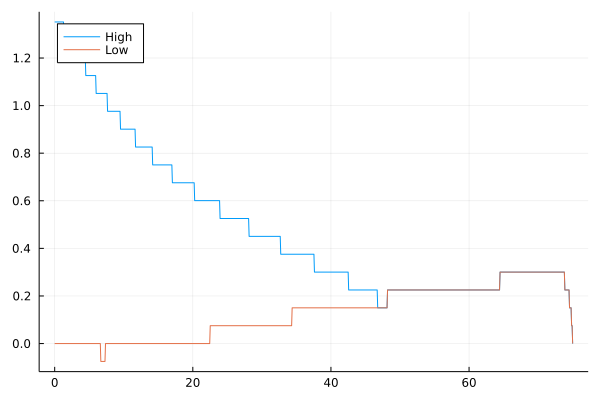
\includegraphics[width=.8\linewidth]{./julia/sav_func_20.png}
	\end{center}
\end{itemize}
~\\
~\\

\section*{Exercise 2}

\begin{itemize}
	\item The steady-state distribution of agents over age, productivity, and asset holdings, $F_{j}(z, a)$, is computed in the julia code.
	
\end{itemize}

\pagebreak

\section*{Exercise 3}
\begin{itemize}
	\item Results of policy experiments are presented below.\\

	

		\begin{tabular}{l|l|l|l|l|l|l} 
			\hline
			& \multicolumn{2}{l|}{Benchmark} & \multicolumn{2}{l|}{No risk} & \multicolumn{2}{l}{Exogenous labor}  \\ 
			\hline
			& with SS & without SS           & with SS & without SS         & with SS & without SS                 \\ 
			\hline
			capital ($K$)         & 3.348   & 4.604                & 1.078    & 1.312              & 7.348   & 10.421                     \\ 
			labor ($L$)           & 0.341   & 0.364                & 0.164   & 0.167              & 0.753   & 0.753                      \\ 
			wage ($w$)            & 1.456   & 1.595                & 1.263   & 1.344              & 1.455   & 1.648                      \\
			interest ($r$)        & 0.024   & 0.011                & 0.048   & 0.036              & 0.024   & 0.007                      \\
			pension benefit ($b$) & 0.225   & 0.0                  & 0.093   & 0.0                & 0.493   & 0.0                        \\
			total welfare ($W$)   & -35.8   & -37.3                & -44.9   & -45.2              & -23.1   & -25.8                      \\
			cv(wealth)        & 0.598   & 0.673                & 1.282   & 1.074              & 0.603   & 0.707                      \\
			\hline
		\end{tabular}
\\
~\\
\begin{itemize}
	\item[1.] After eliminating social security, aggregate capital increases from $3.348$ to $4.604$, because households save more in their working ages for the life after retirement. Aggregate labor also increases (from $0.341$ to $0.364$), because labor tax ($\theta$) is removed. The economy-wide welfare decreases from $-35.8$ to $-37.3$ and overall inequality measured by the coefficient of variation of wealth increases (from $0.598$ to $0.673$).
	
	\item[2.] Without idiosyncratic risk (i.e., $z_{High} = z_{Low} = 0.5$), aggregate capital decreases from $3.348$ to $1.078$. This is because households have no motivation to insure against idiosyncratic income risks. After the removal of social security again, the economy-wide welfare slightly decreases from $-44.9$ to $-45.2$. Given that the absolute amount of decrease is far less than that of the benchmark, we can conclude that social security serve the role of an insurance device against idiosyncratic risk. Also, it should be noted that the welfare comparisons across steady states could be misleading, because the impact of reform during the transition period is ignored. 
	
	\item[2.] Finally, we consider exogenous labor supply case. We can see aggregate labor is $0.753$, indicating all agents in their working ages provide 1 unit of labor. Since labor supply is exogenously determined, social security system has no distortionary effect on labor supply. Still, aggregate welfare decreases when social security is eliminated, leading us to the same conclusion as before.
\end{itemize}
\end{itemize}

	
\end{document}